% !TEX encoding = UTF-8
% !TEX TS-program = pdflatex
% !TEX root = ../Tesi.tex
% !TEX spellcheck = en-EN

%************************************************
\chapter[Experimental Characterization]{Experimental Characterization}
\chaptermark{Experimental}
\label{cap:experimentalcharacterization}
%************************************************

\improvement{Add some details for experimental characterization}



\section{Particle Distribution}
\label{sec:particledistribution}

\improvement{Make a table with the particles diameter distributions of all
materials.}

\section{Drained angle of repose (p-p) - small scale}
\label{sec:aor}

\improvement{explain that the values collected refers to particle-particle
interactions} 
A sample was deposited on a 20 cm diameter plate with liftable
boundary called static angle of repose (\acs{AoR}) tester, see Fig. \ref{fig:088aorexperimental}.
Once the particles were in position, the boundary was lifted, allowing some particles to drop. 
Once stabilized, the \acs{AoR} was measured eight times using a digital protractor at different positions of the heap. 
The average of the measurements gave the fourth bulk value (see Table
\ref{tab:14bulkvalues}).
Note that, since the experiments were performed only for relatively large size
bulk solids, the compaction condition in the initial state was not critical to the
final result of this test.\\
\begin{figure}[htbp]
\centering 
  \subfloat[Drained angle of repose.]{
	  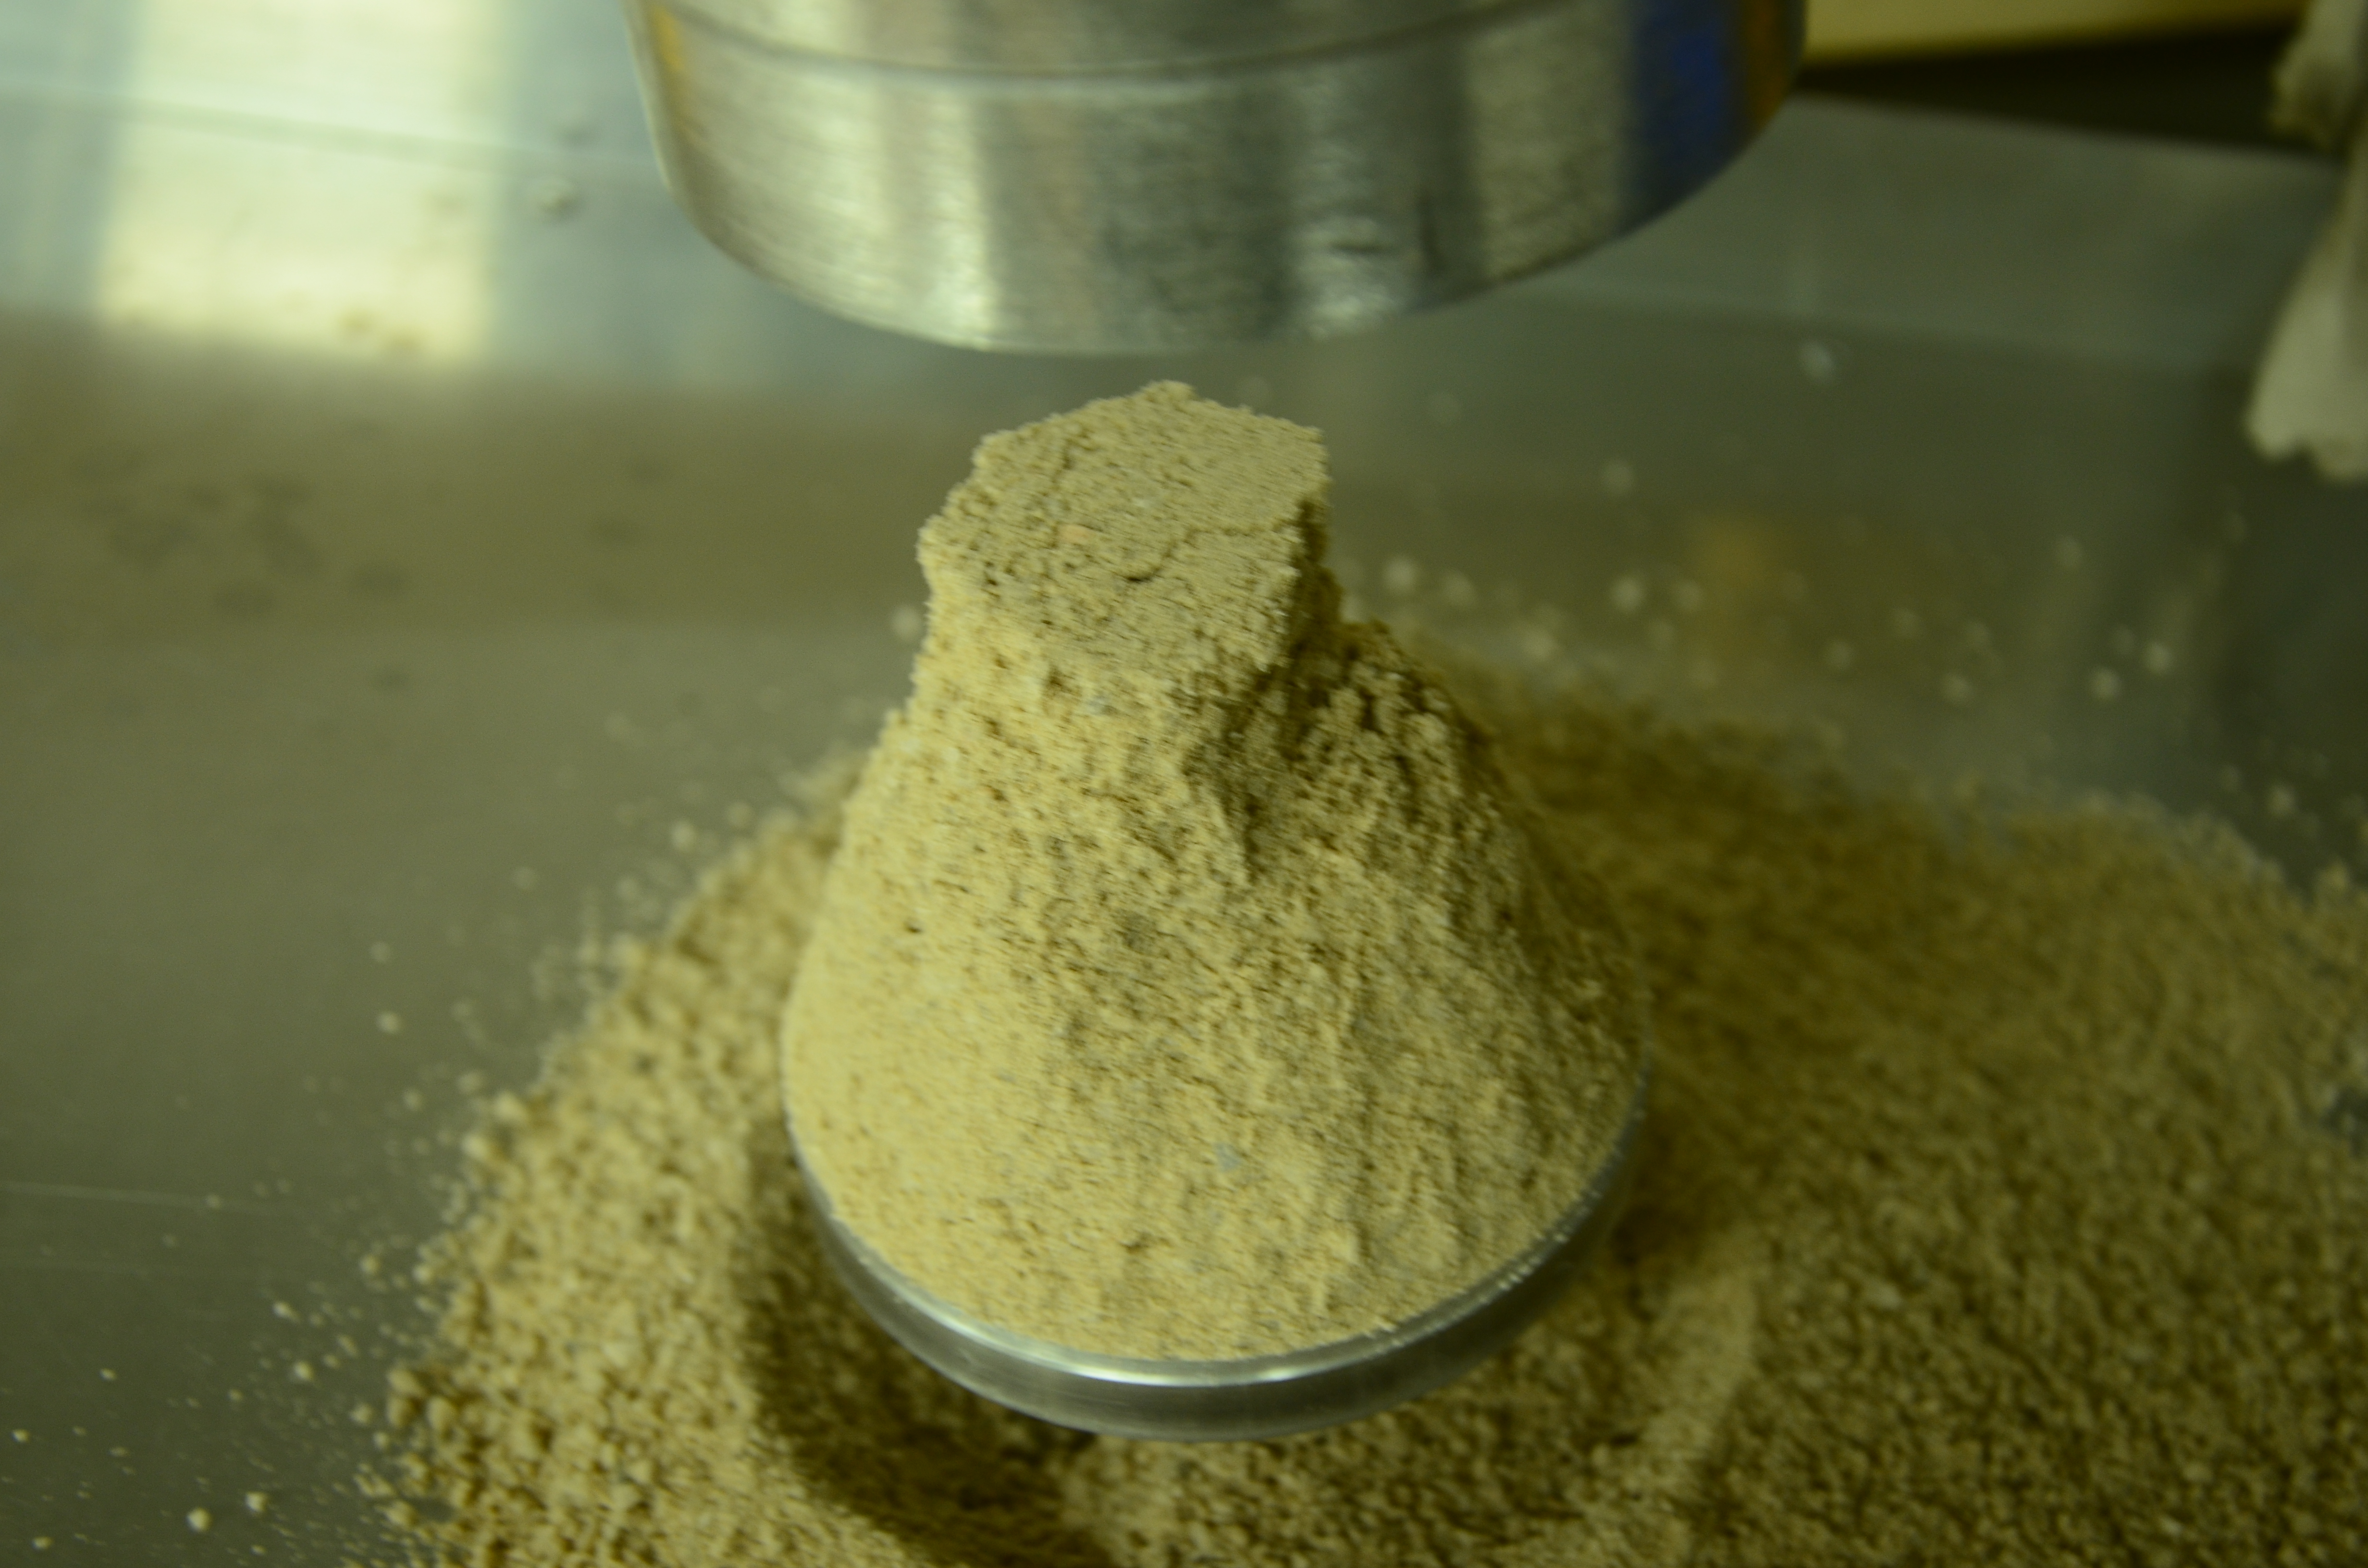
\includegraphics[width=.54\columnwidth]{images/051aorLab}
	  \label{fig:051aorLab}
  }
  \quad
    \subfloat[Drained angle of repose tester.]{
	  \includegraphics[width=.40\columnwidth]{images/005aor}
	  \label{fig:005aor}
  }
  \\
  \caption{AoR experimental tester.}
  \label{fig:088aorexperimental}
\end{figure}

\section{Drained angle of repose (p-p) - large scale}
\label{sec:aorlargescale}

At the Leoben VAS facility a new rotating double chute was used: 
nine large scale dynamic angle of repose tests were performed. 
\improvement{Evaluate large-small scale AoR relationship and put some images.}

\section{Jenike Shear Cell tester}
\label{sec:jsct}
%************************************************

\improvement{Write something about JSCT (simplified version of RSCT, or
viceversa).}
Fig. \ref{fig:052ShearCellLab} \\
Fig. \ref{fig:053PoorMan} \\
Fig. \ref{fig:003sjsct} \\

Fig. \ref{fig:004sjsctdiagram} \\
\begin{figure}[htbp]
\centering 
  \subfloat[Laboratory setup of the Jenike shear cell tester.]{
	  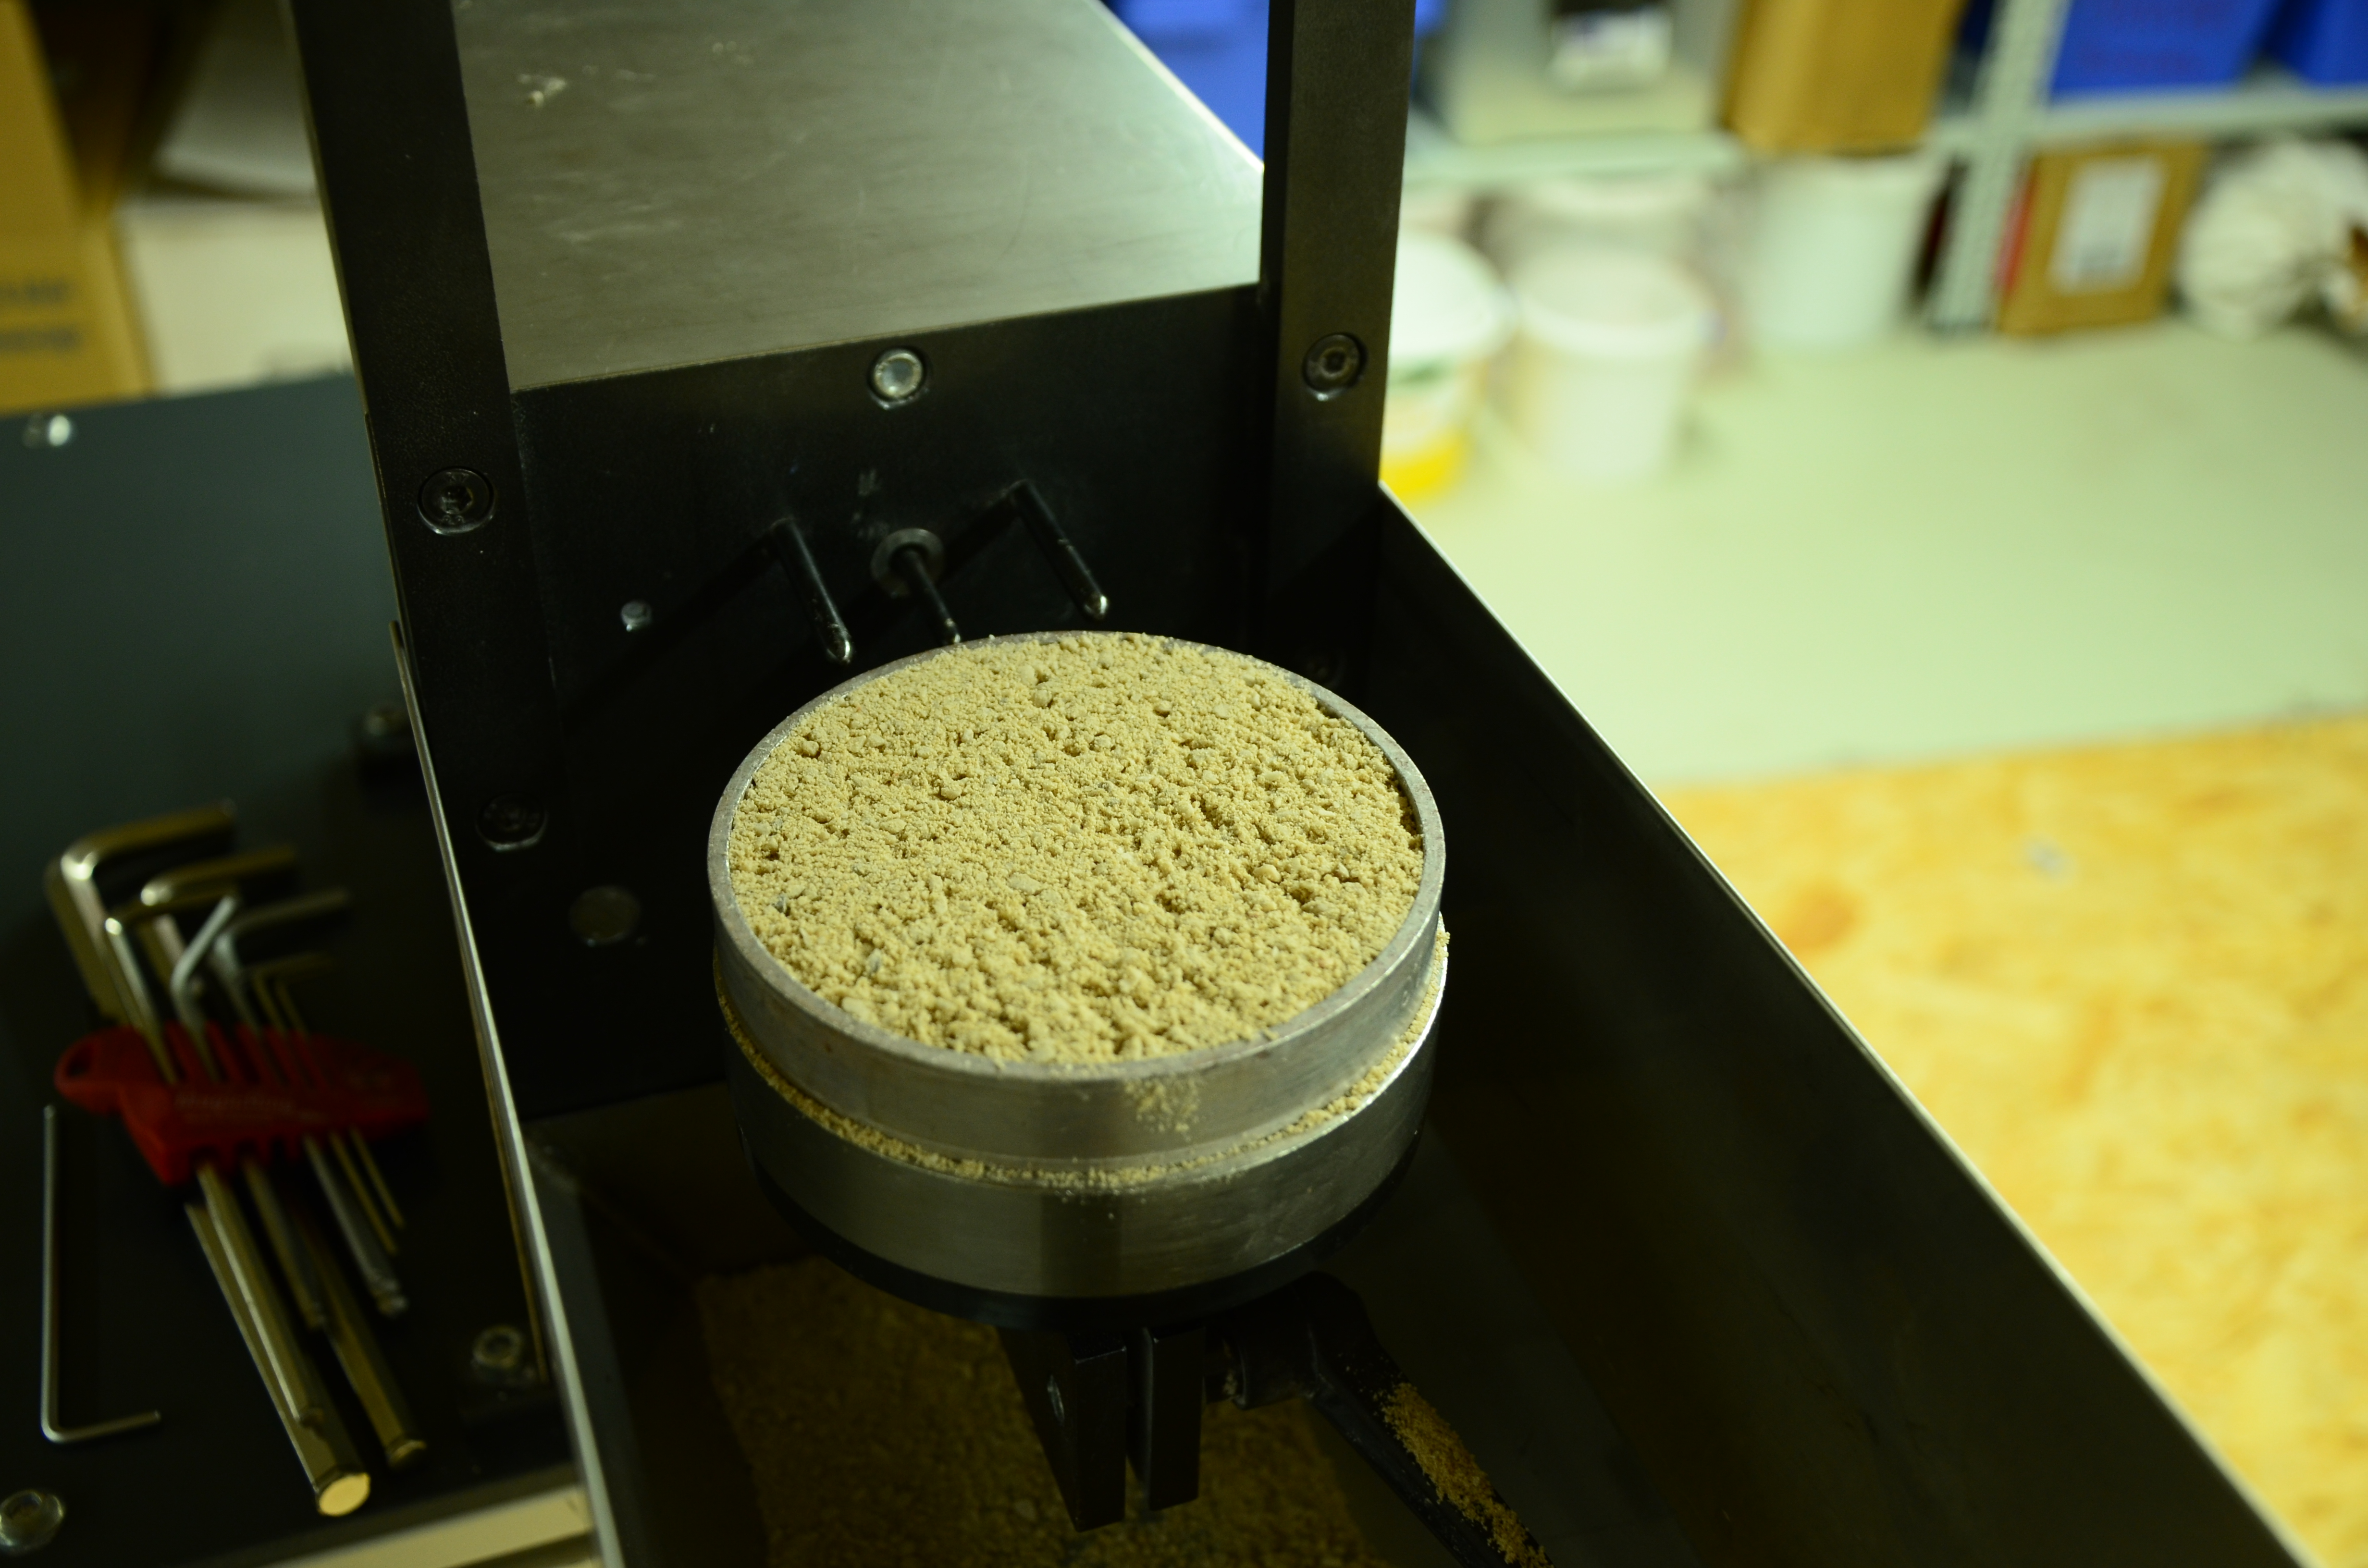
\includegraphics[width=.44\columnwidth]{images/052ShearCellLab}
	  \label{fig:052ShearCellLab}
  }
  \quad
    \subfloat[Laboratory setup of the simplified Jenike shear cell tester.]{
	  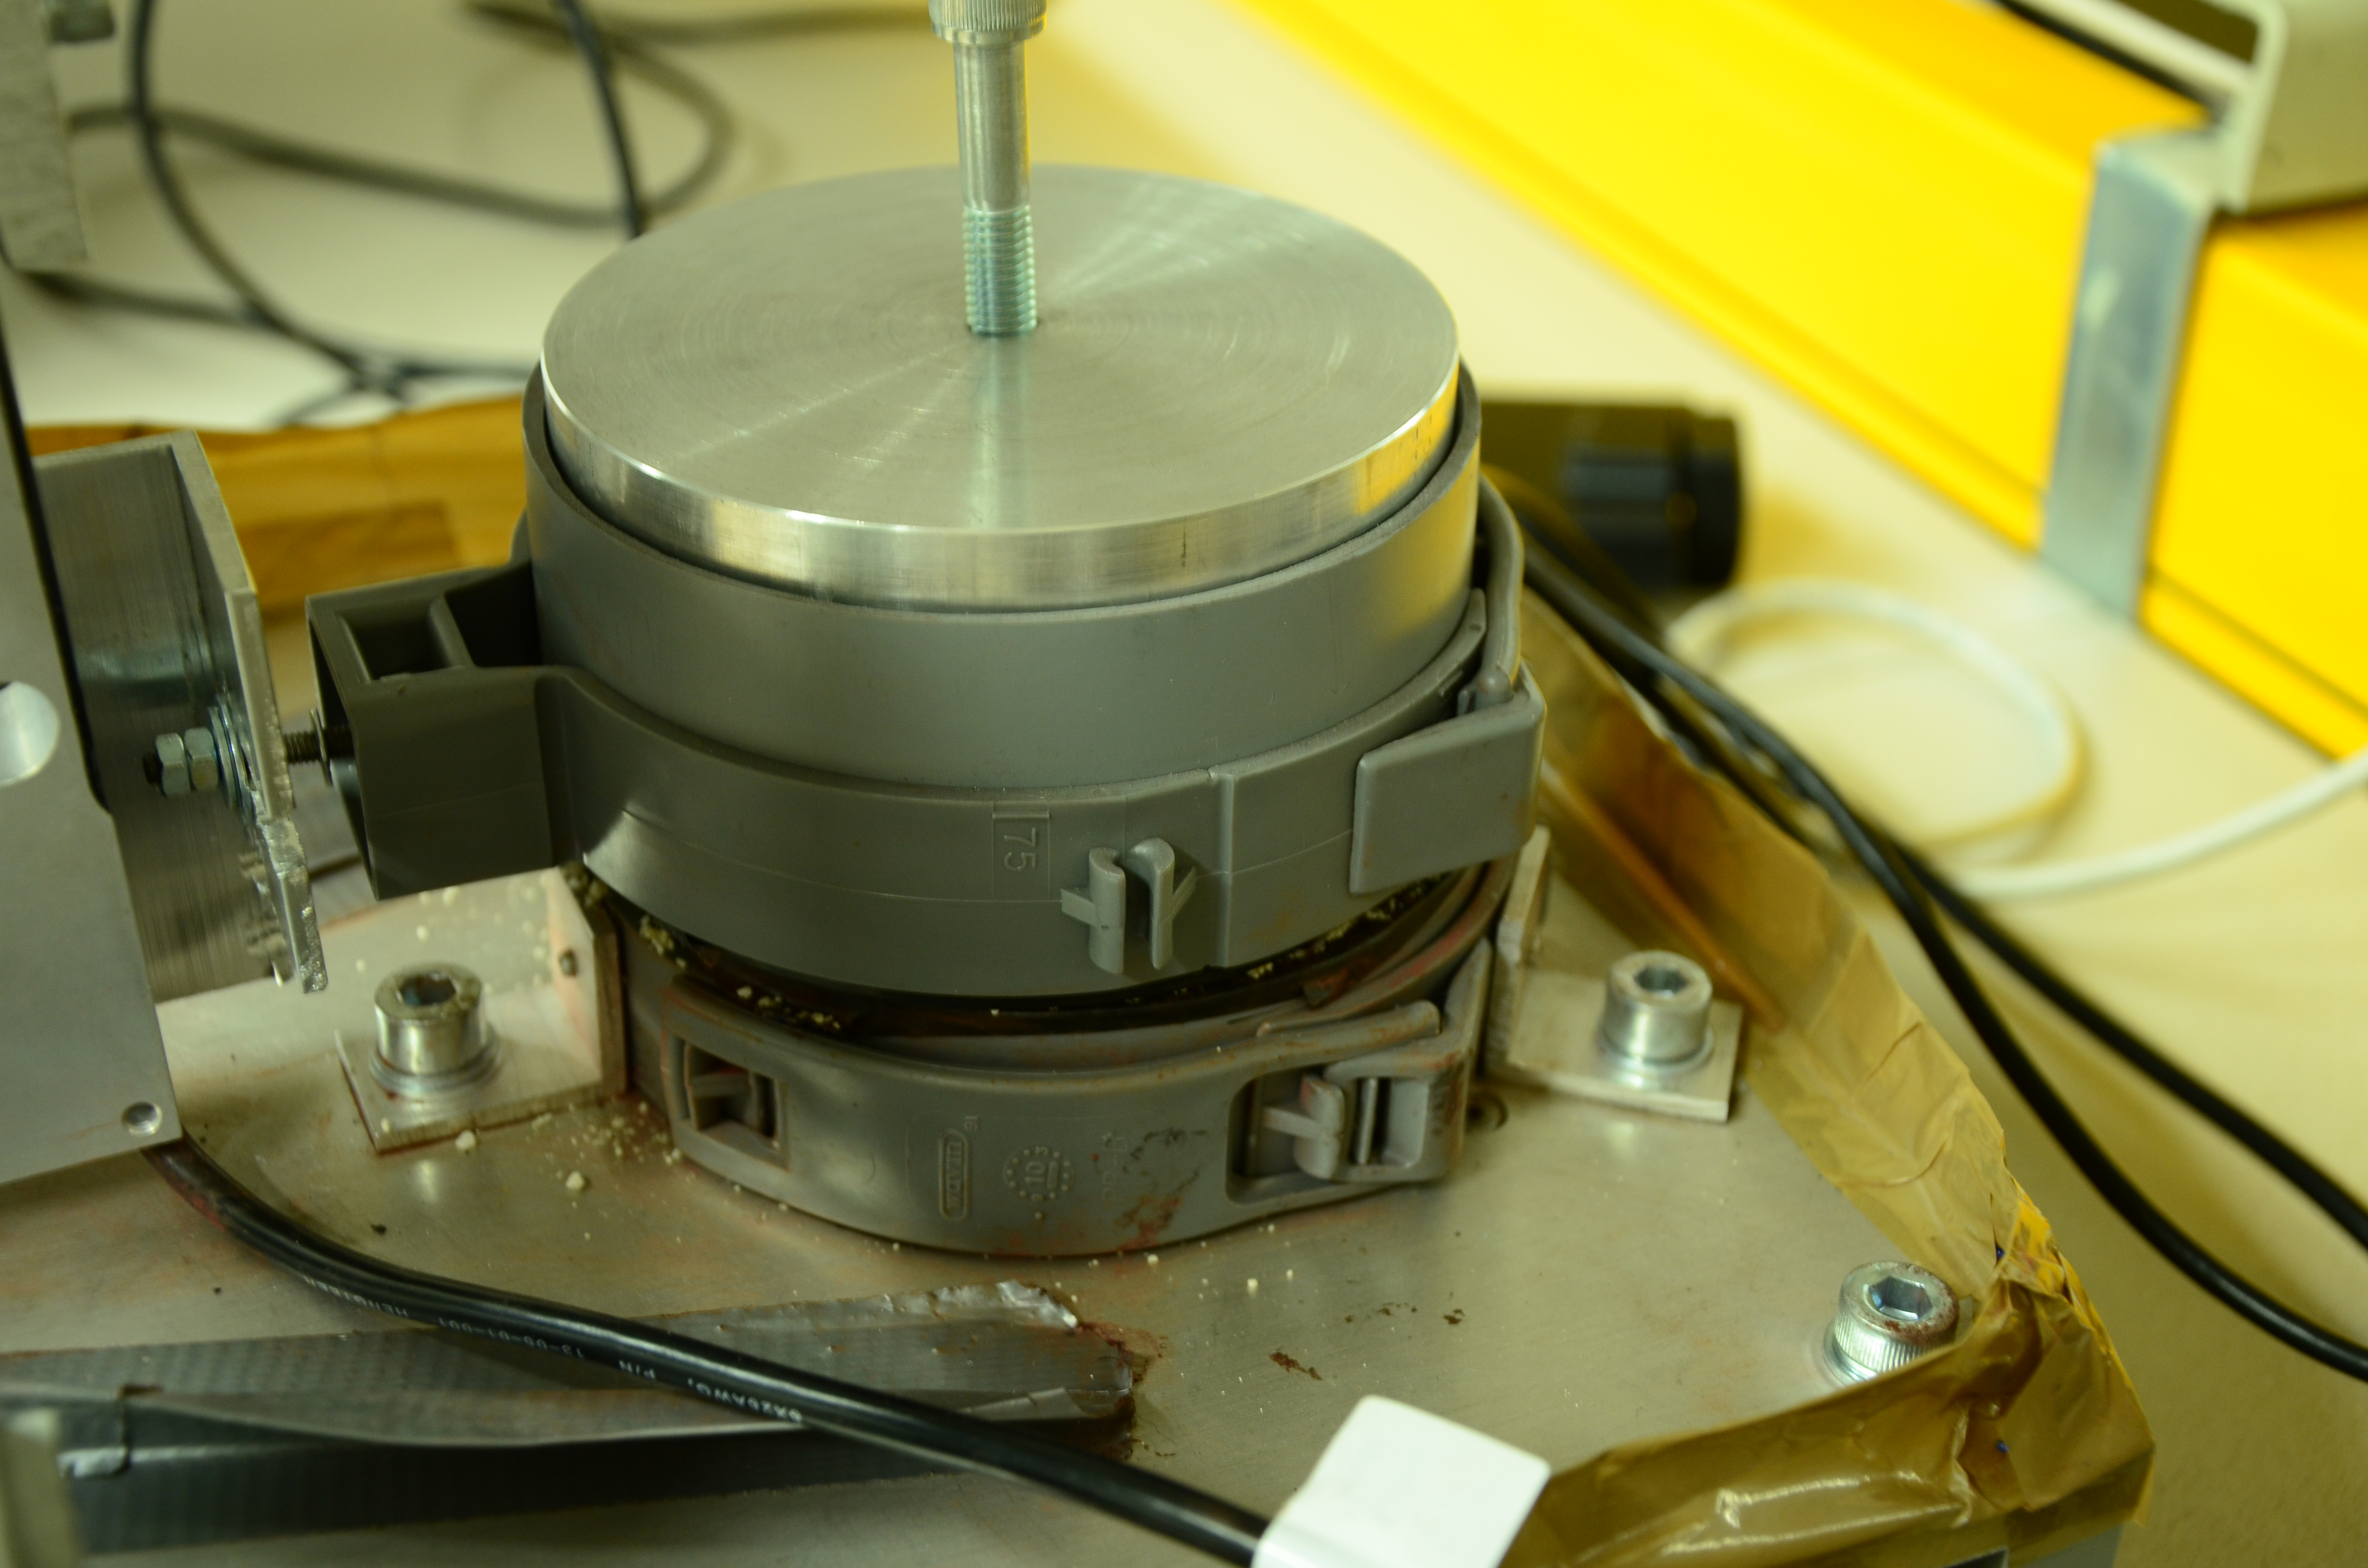
\includegraphics[width=.44\columnwidth]{images/053PoorMan}
	  \label{fig:053PoorMan}
  }
  \\
  \subfloat[Jenike shear cell tester layout \cite{RefWorks:69}.]{
	  \includegraphics[width=.44\columnwidth]{images/003sjsct}
	  \label{fig:003sjsct}
  }
  \quad
    \subfloat[Jenike shear cell tester diagram of the shear stress, on the y axis,
    over time, on the x axis \cite{RefWorks:69}.]{
	  \includegraphics[width=.44\columnwidth]{images/004sjsctdiagram}
	  \label{fig:004sjsctdiagram}  }
  \\
  \caption{JSCT.}
  \label{fig:089jsctexperimental}
\end{figure}

\section{Schulze Ring Shear Cell tester (p-p)}
\label{sec:SRSCT}
%************************************************

\begin{figure}[htbp]
\centering 
  \subfloat[Ring shear cell tester layout.]{
	  \includegraphics[width=.40\columnwidth]{images/001srsct}
	  \label{fig:001srsct}
  }
  \quad
    \subfloat[Ring shear cell diagram of the shear stress, on the y axis,
    over time, on the x axis.]{
	  \includegraphics[width=.54\columnwidth]{images/002srsctdiagram}
	  \label{fig:002srsctdiagram}
  }
  \\
  \caption[SCT experimental tester.]{SCT experimental tester
  \cite{RefWorks:69}.}
  \label{fig:090sctexperimental}
\end{figure}

A representative sample of bulk solid was placed in a Schulze ring shear cell
tester (\acs{SCT}) of specified dimensions ($external ~ radius = 100 ~ mm$,
$internal ~ radius = 50 ~ mm$), see Fig. \ref{fig:001srsct}.
A normal load was applied to the cover. As soon as the lid touched the sample,
its position was calculated.
Together with the area of the ring, the total volume can be calculated, and subsequently the 
\textit{bulk density} \acs{rhob}, the first bulk value
of the sample, was obtained.
Later, we tried to obtained the \textit{bulk values} indicated in Table
\ref{tab:14bulkvalues}, slightly different from those indicated in Fig.
\ref{fig:002srsctdiagram}.
A representative stress path can be seen in Fig. \ref{fig:020experimental}.
Time was normalized: $\tilde{t} = t/t_{change}$, where $t_{change}$ is the
point in time at which the normal stress (\acs{sigman}) was modified during the	tests.
After the \acs{rhob} identification, the \acs{sigman} was kept constant at e.g.
10,000 Pa until $\tilde{t}=1$.
The specimen was in this way pre-sheared until a steady-state shear value was
reached from $\tilde{t}~=0.91$ to $\tilde{t}=1$.
The steady-state flow horizontal stress
is called steady-state flow/pre-shear stress.
If the normal stress is known, it provides (Eq. \ref{eq:phi_ps}) the angle of
internal friction of the pre-shear phase ($\phi_{e-psh}$), and consequently the
pre-shear coefficient of internal friction $ (\mu_{psh})$, the second
bulk value, see Schulze \cite{RefWorks:118}:
%************************************************
\begin{equation}
\begin{aligned}
\phi_{e-psh} &= \arctan \left(\frac{\tau_{psh}}{\sigma_{n,psh}} \right) ,\\
\mu_{psh} &=\tan(\phi_{e-psh}) .
\end{aligned}
 \label{eq:phi_ps}
\end{equation}

%************************************************
At $\tilde{t}=1$ the normal stress and the angular velocity were then
immediately reduced to zero.
Subsequently, the specimen was sheared under a fraction (\acs{tauperc})(e.g.
80\%) of the first normal load until the shear force reached a a second plateau.
Both the pre-shear and shear phases were executed at constant velocity. 
We define the horizontal stress at the shear force peak as the average shear
stress in this second plateau, thus obtaining the incipient flow/shear
coefficient of internal friction \acs{mush}, third bulk value (Eq. \ref{eq:phi_s})\cite{RefWorks:118}:
%************************************************
\begin{equation}
\begin{aligned}
\phi_{e-sh} &= \arctan \left(\frac{\tau_{sh}}{\sigma_{n,sh}} \right) ,\\
\mu_{sh} &= \tan(\phi_{e-sh}) .
\end{aligned}
 \label{eq:phi_s}
\end{equation}

%************************************************
Three different pre-shear normal loads were applied in the experiment
(1,000, 2,000, and 10,000 Pa).
For each we used a normal load proportional to the initial one
(\acs{tauperc}), increasing from stage one (40\%) to stage four (100\%)
with two escalating intermediate stages (60\% and 80\%) for a total of twelve load conditions.
Each experiment was performed on a fresh material sample. \\
\begin{figure}[!htb] 
\centering 
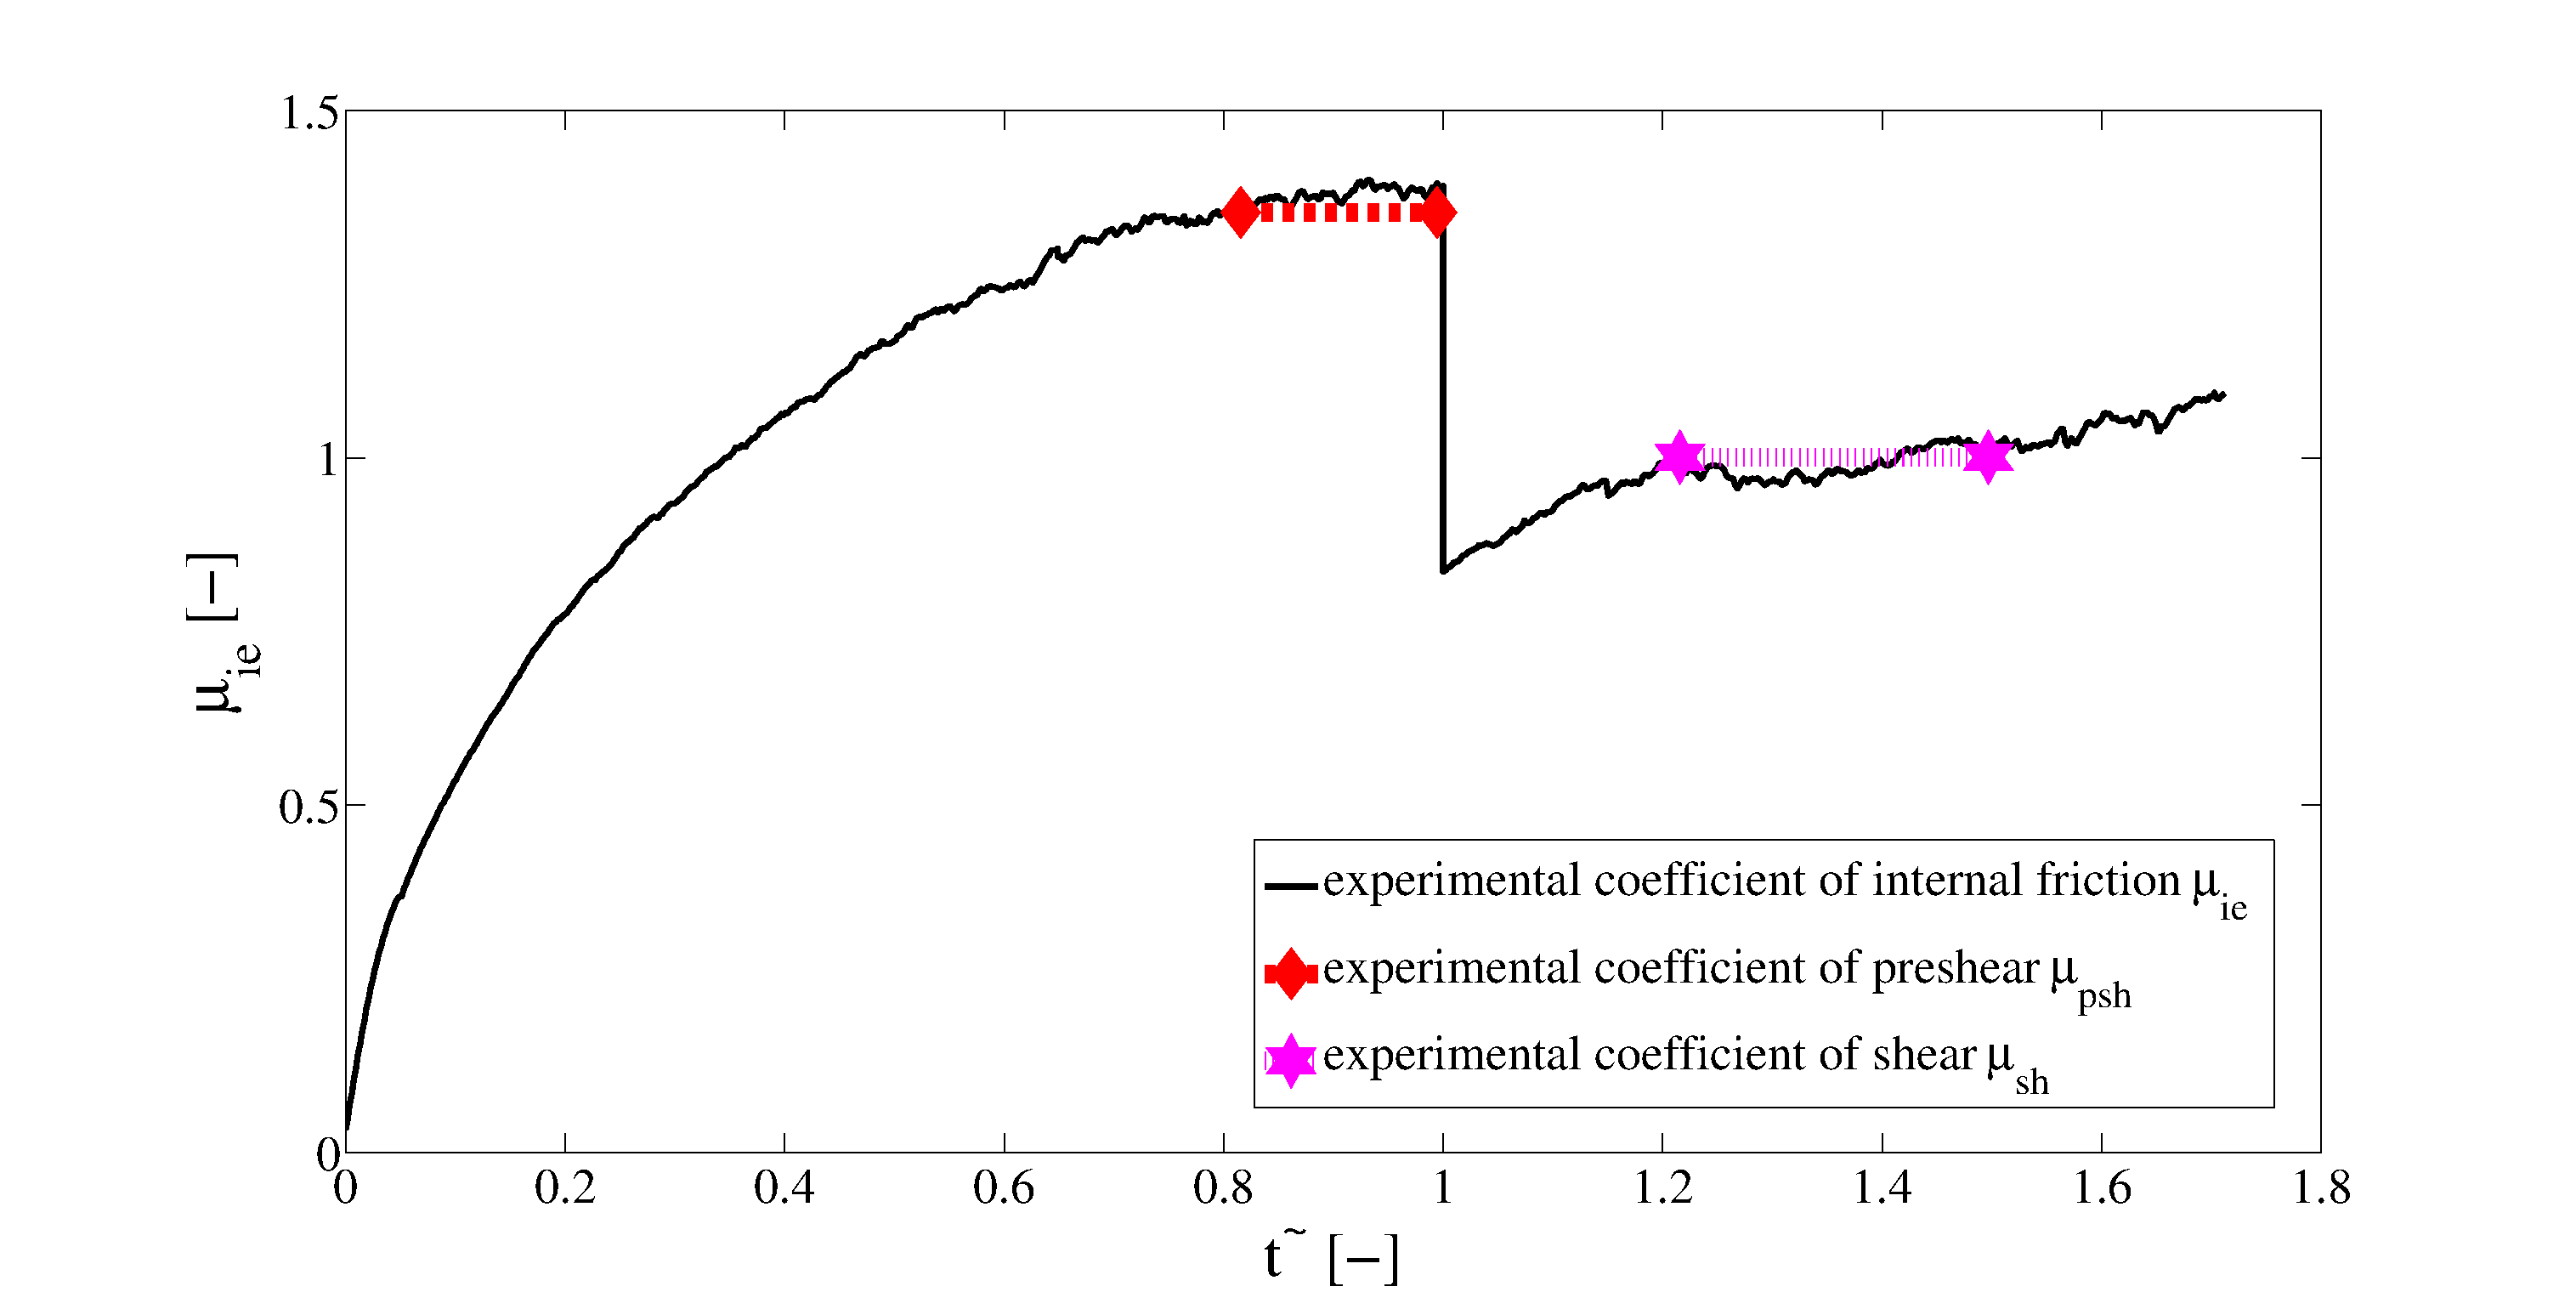
\includegraphics[width=.96\textwidth]{images/020experimental} 
\caption[Experimental shear cell tester stress path]{Experimental shear-cell tester stress path - $\sigma_n = 10000
        ~Pa$.}
\label{fig:020experimental} 
\end{figure}

% \begin{figure}[htp] \centering
%     \begin{subfigure}[b]{0.96\columnwidth}
%         \includegraphics[width=\textwidth]{20experimental}
%         \caption{Experimental shear-cell tester stress path - $\sigma_n = 10000
%         ~Pa$}
%         \label{fig:20experimental} 
%     \end{subfigure}\\
%         \begin{subfigure}[b]{0.96\columnwidth}
%         \includegraphics[width=\textwidth]{21simexample}
%         \caption{Numerical shear-cell tester stress path - $\sigma_n = 10000
%         ~Pa$}
%         \label{fig:21simexample} 
%     \end{subfigure}
%     \caption[Stress path]{Experimental and numerical samples of the stress path
%     for the Schulze ring shear cell tester.
% 	Time was normalized: $\tilde{t} = t/t_{change}$, where $t_{change}$ is the
% 	point in time at which the normal stress ($\sigma_n$) was modified during the
% 	tests.
% 	Until $\tilde{t}=1$, the $\sigma_n$ was kept constant at 10,000 Pa. 
% 	In Fig. \ref{fig:20experimental}, 
%  	a plateau was reached at $\tilde{t}~=0.91$.
% 	The coefficient of pre-shear ($\mu_{psh}$) was calculated as the average of the
% 	coefficient of internal friction ($\mu_{ie}$) in this first plateau.
% 	At $\tilde{t}=1$, the $\sigma_n$ was reduced to $80 \%$ of its initial
% 	value, and soon after
% 	a second plateau developed.
% 	We obtained the coefficient of
% 	shear ($ \mu_{sh}$) as the average of $\mu_{ie}$ in this second plateau.
% 	The stress paths agree well, especially the plateaux.
% 	They were clearly relevant because
% 	the values representative of the bulk behaviours 
% 	were collected there.}
%     \label{fig:40experimentalsimulation}
% \end{figure}
The stress paths between Fig. \ref{fig:007shearcellsim} and Fig.
\ref{fig:020experimental} agree well, especially the plateaux.
They were clearly relevant because
the values representative of the bulk behaviours were collected there.

% \section{Parameter Identification}
% \label{sec:parameteridentification}
% 
% We obtained for each of the twelve load conditions of the \acs{SCT} three bulk
% values (\acs{mupsh}, \acs{mush} and \acs{rhob}).
% The fourth bulk value was the result of two angle of repose (\acs{AoR}) tests that
% recreated the repose angle observed in a pile of the
% real material. 
% Subsequently, we compared the \acs{ANN} and experimental bulk behaviours for the
% twelve shear-cell load conditions.
% If in a DEM-parameter combination all the three bulk values differed by less 
% than 5\% from those of the corresponding experiments, i.e.:
% %************************************************
%  \begin{equation}
 \begin{cases}
\text{if } & \lvert{1-\frac{\mu_{psh,num}}{\mu_{psh,exp}}}\rvert < 5\%  ,\\
\text{and if } & \lvert{1-\frac{\mu_{sh,num}}{\mu_{sh,exp}}}\rvert < 5\% , \\ 
\text{and if } & \lvert{1-\frac{\rho_{p,num}}{\rho_{p,exp}}}\rvert < 5\% ,\\ 
\end{cases}
 \label{eq:check2}
\end{equation}

% the combination was marked. The marked combinations were processed by the
% \acs{AoR} \acs{ANN}, and then compared with the experiment.
% Were considered valid those that differed by less than $5\%$ also in this
% comparison (Eq. \ref{eq:checkaor}):
% %************************************************
% \begin{equation}
\text{if} ~~~~~~ \lvert{1-\frac{AoR_{num}}{AoR_{exp}}}\rvert < 5\% .
\label{eq:checkaor}
\end{equation}
%************************************************
% Further, to prove the validity of the system, we tested the marked combinations
% by modifying the experimental bulk values of the shear cell. 
% We artificially decreased or increased the shear force, and thus \acs{mupsh} and
% \acs{mush}, by a product coefficient ($P$), e.g. Eq. \ref{eq:pcoeff}:
% %************************************************
% \begin{equation}
\label{eq:pcoeff}
\mu_{psh, new} = \mu_{psh, old} \cdot P .
\end{equation}
%************************************************
% 
% \subsection{Value representation}
% \label{subsec:valuerepresentation}
% 
% \begin{itemize}
%   \item{parameter space plot;}
%   \item{box plot;
%   \improvement{explain about 25 and 75 percentile}
%   }
%   \item{density plot.}
% \end{itemize}